\begin{figure*}[t!]
    \centering
        \begin{subfigure}[b]{\linewidth}
        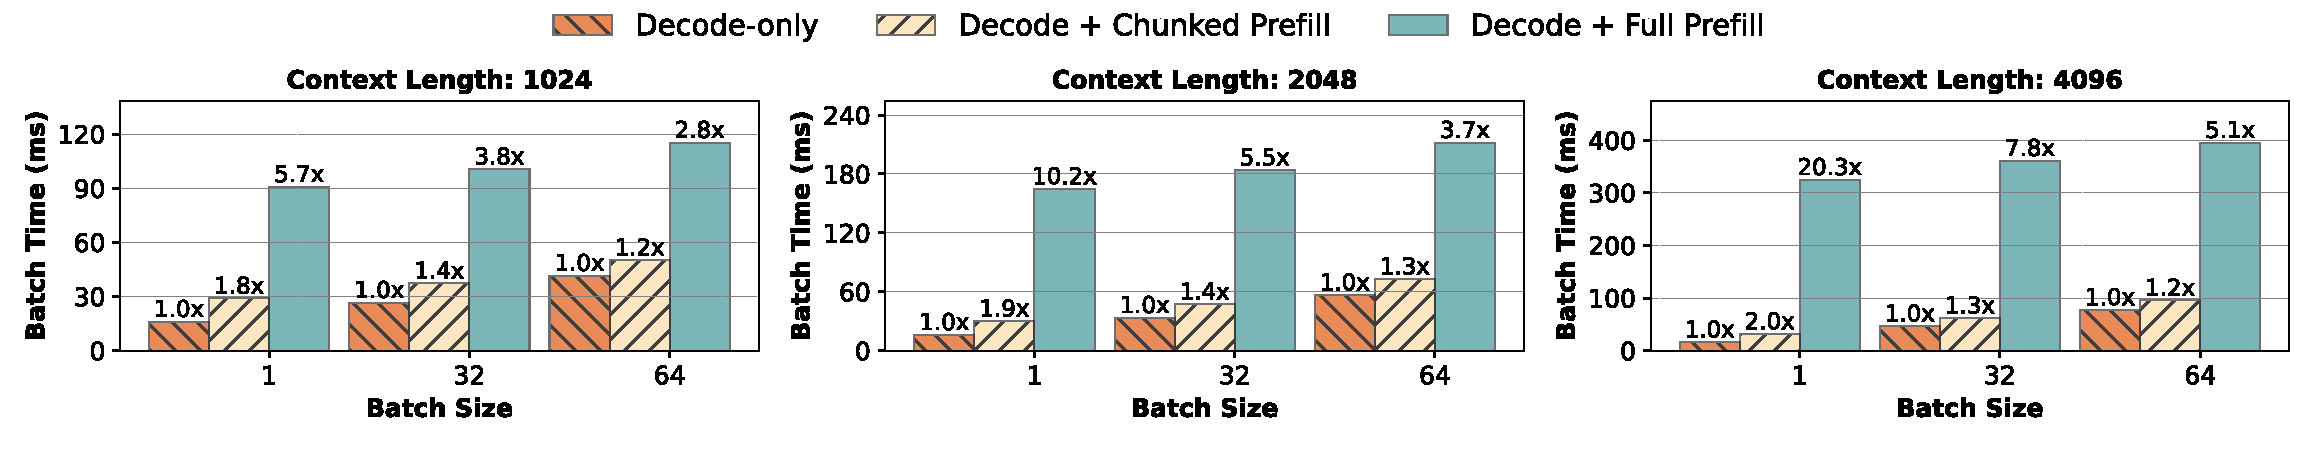
\includegraphics[width=\linewidth]{figures/piggybacking_cost_mistral_7b_1.pdf}
        \caption{Mistral-7B on one A100s with token budget of 256.}
        \label{fig:motivation:incrementalcost:mistral}
    \end{subfigure}
    \\
    \begin{subfigure}[b]{\linewidth}
        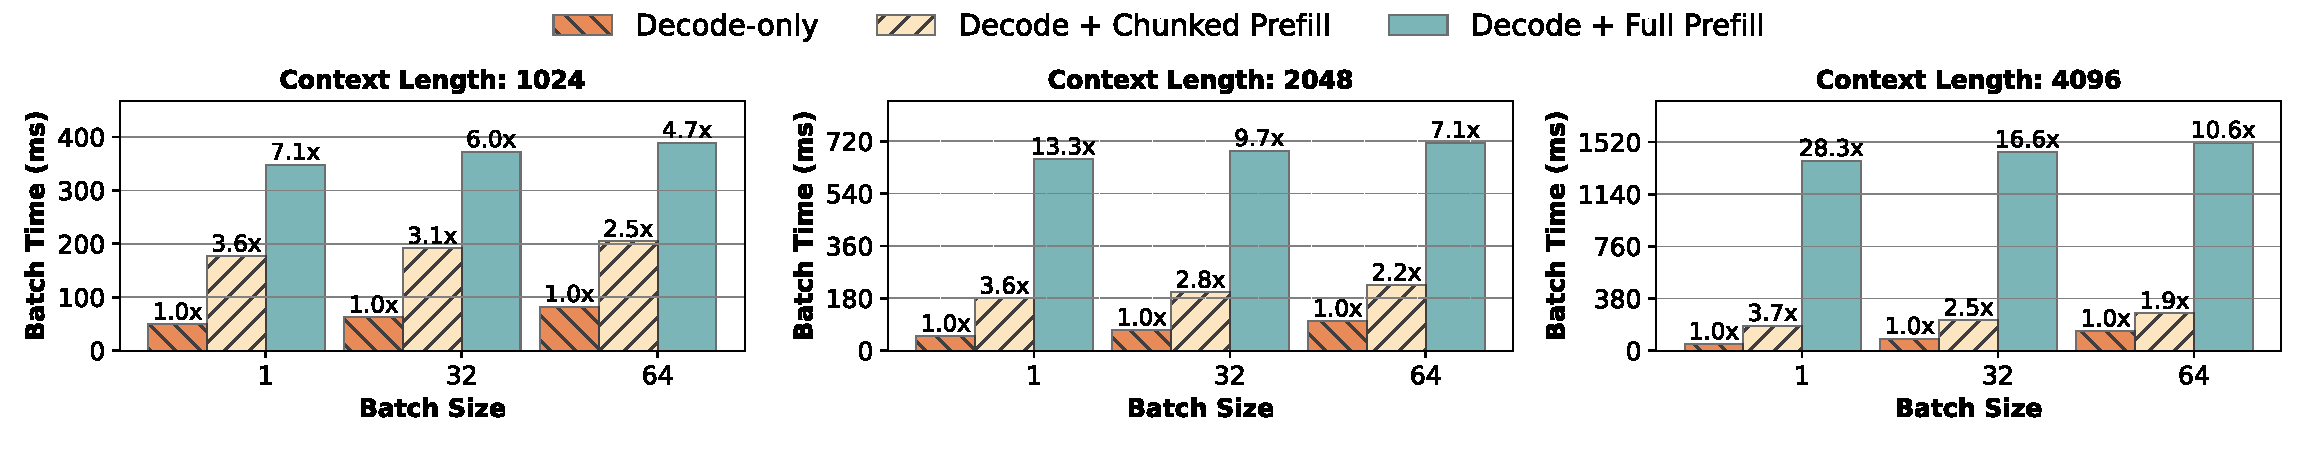
\includegraphics[width=\linewidth]{figures/piggybacking_cost_llama_70b_1.pdf}
        \caption{\llamaL on four A100s with token budget of 512.}
        \label{fig:motivation:incrementalcost:llama}
    \end{subfigure}

    \caption{The incremental cost of coalescing prefills with decode batches. We consider two batching schemes -- (i) Decode + Full Prefill represents the hybrid batching of Orca wherein the entire prefill is executed in a single iteration along with ongoing decodes. (ii) Decode + Chunked Prefill represents \sysname wherein prefills are chunked before being coalesced with ongoing decodes with a fixed token budget. \sysname processes prefill tokens with much lower impact on the latency of decodes. Further, the relative impact of \sysname on latency reduces with higher decode batch size and context lengths.}
        \label{fig:motivation:incrementalcost}
\end{figure*}
